\section{Introduction}


% Preface paragraph
%Rapid technological advancements are embedded into multiple aspects of our everyday life.  Digital processing of information has enabled great levels of automation enhancing our quality of life. These advancements allow us to capture, share, and consume footage of our or other's everyday experiences. The definition of algorithms able to \emph{understand} these experiences and the actions performed has been of particular interest to the computer vision community since its early days. 
For decades analyzing human actions in videos has been of particular interest to the computer vision community. Videos are prominent in both our social and professional everyday lives. The analysis of actions has shifted from the well-understood task of action recognition towards the fundamental and broader area of action understanding. The unique challenges and novel computation tasks of action understanding are the core focus of our survey. 

% Action understanding in cognitive science 
In developmental psychology, action understanding has been explored across several psychological aspects \citep{thompson2019conceptualizing}: 

\noindent
\textbf{The ability to understand the action performed} relates to differentiating between analogous actions \citep{gallese1996action,jeannerod1994representing} and conceptualizing \emph{how} an action is performed \citep{spunt2011identifying}. 

\noindent
\textbf{Determining the goal of the action} has been studied in the context of immediate goals \citep{calvo2005action,kohler2002hearing,rizzolatti2001neurophysiological}, in terms of the motor functions for the execution of actions and the sensory perception of actions performed by others.

\noindent
\textbf{Determining the actor's intention} refers to identifying high-level motivations for performing actions \citep{kilner2011more}. Intentions have been defined as the sequential grouping of individual actions \citep{fogassi2005parietal} and their abstract associated target \citep{uithol2011understanding}.

\begin{figure*}[t]
    \centering
    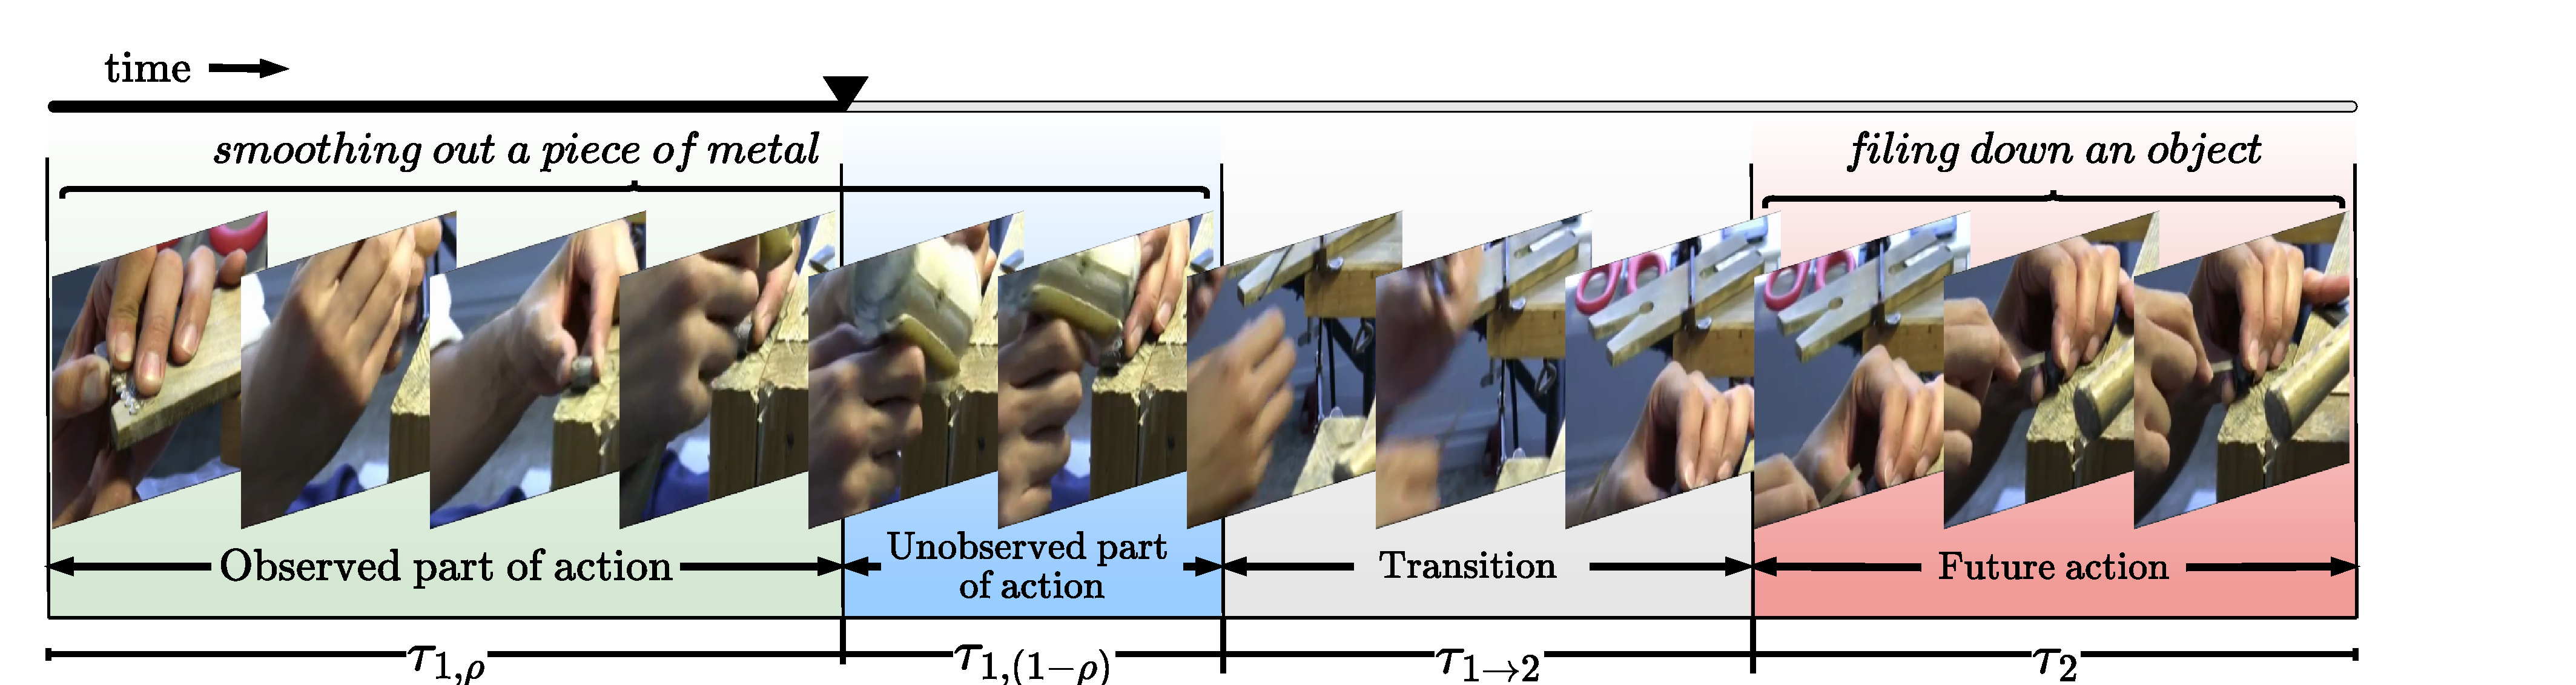
\includegraphics[width=\linewidth,trim={1cm 0 6cm 0},clip]{figs/action_understanding_tasks.pdf}
    \caption{\textbf{Action understanding tasks}. The progress of the video is indicated by the top bar. From the currently performed action of total duration $\tau_1$, only the $\tau_{1,\rho}<\tau_1 $ part is readily observable. After a transition period $0\leq\tau_{1 \rightarrow 2}$, another action is performed with duration $\tau_2$. \textbf{Action recognition} tasks consider full observations of the action at $\tau_1$. \textbf{Action prediction} uses only part $\tau_{1,\rho}$ of the ongoing action. \textbf{Action forecasting} uses current action at $\tau_1$ to predict future actions. Video example sourced from \citet{wang2019vatex}.} 
    \label{fig:tasks}
\end{figure*}

\subsection{Taxonomy of this survey}

% Temporal scopes
Inspired by the cognitive aspects of action understanding, we define three broad \emph{temporal scopes} and respectively group seminal machine vision action understanding tasks. We visualize action sequence progression in~\Cref{fig:tasks} with a currently (partially) performed action followed by a subsequent action. Tasks that require all actions to be \emph{observed in full} are broadly referred to as \textbf{recognition} tasks and infer information such as the action categories or high-level semantics. \textbf{Predictions} about the ongoing actions are made from partial observations of actions \emph{not yet completed}. \textbf{Forecasting} tasks use the currently observed action(s) to reason future actions \emph{not yet observed}.  We discuss relevant previous surveys for each of these three temporal scopes and overview their research focus' in \Cref{tab:surveys}.

\noindent
\textbf{Recognition}. Early works on action recognition have primarily focused on motion modeling. \citet{aggarwal1994articulated} used a taxonomy of rigidness and subsequently \citep{aggarwal1998nonrigid} introduced subdivisions based on prior knowledge of the object's shape. \citet{cedras1995motion} and later \citet{moeslund2001survey} discussed temporal modeling approaches in the context of classification and tracking. As overviewed by \citet{buxton2003learning}, tracking had also been applied to more complex tasks such as behavior analysis or non-verbal human interactions, with divisions also discussed by \citet{poppe2007vision}. 
% Classification surveys
More explicit scopes such as action classification and localization \citep{weinland2011survey}, behavior understanding \citep{chaaraoui2012review}, or surveillance applications \citep{vishwakarma2013survey} emerged based on later advancements. These surveys explored task-specific methods and more semantically complex topics. \citet{turaga2008machine} and \citet{poppe2010survey} discussed approaches addressing atomic actions and group activities. \citet{herath2017going} provided an initial summary of approaches using learned features for action recognition. Following surveys overviewed adaptations of deep learning approaches for topics such as depth-based motion recognition \citep{wang2018rgb}, activity recognition \citep{beddiar2020vision}, human-human interactions \citep{stergiou2019analyzing}, and pose estimation \citep{zheng2020deep}. \citet{sun2022human} reviewed approaches across multiple modalities, combining motion features, audio, and vision. More recently, \citet{selva2023video} discussed attention-based approaches for video tasks while \citet{schiappa2023self} focused on self-supervised (SSL) approaches. \citet{madan2024foundation} also presented a comprehensive overview of video foundation models for multiple video understanding tasks.

\noindent
\textbf{Prediction}. Recent advancements in action recognition have also sparked interest in predictive tasks from partial observations. \citet{rasouli2020deep} discussed four main domains of predictive models including video, action, trajectory, and motion prediction. \citet{kong2022human} described recent action recognition and prediction advancements. They focused on applications in domains such as robot vision, surveillance, and driver behavior prediction. The surveys of \citet{dhiman2019review} and \citet{ramachandra2020survey} overviewed predictive methods specifically for anomaly detection.

\noindent
\textbf{Forecasting}. Action forecasting tasks have become prevalent parts of action understanding research. \citet{rodin2021predicting} discussed future action anticipation in egocentric videos. \citet{zhong2023survey} overviewed short and long-term action anticipation methods. \citet{hu2022online} provided a review of online and anticipation works. More recently, \citet{plizzari2024outlook} discussed challenges in egocentric videos and presented future directions for multiple tasks including forecasting.


  
% Addressing multiple aspects of action understanding
Despite their extensive coverage, prior surveys focus on specific aspects of action understanding. As shown in \Cref{tab:surveys}, a critical overview that holistically explores multiple aspects of action understanding is currently missing in the literature. 



\begin{table*}[t]
    \centering
    \caption{\textbf{Action understanding surveys through the years}. For each survey, we identify the coverage of temporal scopes (recognition/Rec., prediction/Pred., forecasting/For.), broad objectives (multi-modality/MM, self-supervision/SSL, multi-view/MV), and specific tasks (human interactions/HI, long video understanding/LVU).%. Scopes/objectives/tasks addressed partially by surveys are denoted with (partial) and the main focus is denoted with \ding{52}.
    }
    \resizebox{\textwidth}{!}{
    \begin{tabular}{l c c c c c l c c c l c c}
    \toprule
    \multirow{2}{*}{Author(s)} & 
    \multirow{2}{*}{Year} &
    \multirow{2}{*}{\#Papers} & \multicolumn{3}{c}{Temporal Scope} & $\;$ & \multicolumn{3}{c}{Objectives} & $\;$ & \multicolumn{2}{c}{Tasks} \bstrut\\ \cline{4-6}\cline{8-10}\cline{12-13}
    & & &
    Rec. & Pred. & For. & $\;$ & MM & SSL & MV & $\;$ & HI & LVU  \tstrut\\
    \midrule
    \citet{aggarwal1994articulated} & 1994 & 
    69 &  
    (partially) & 
      & 
      && 
      & 
      & 
      && 
      & \\
    \citet{cedras1995motion} & 1995 &
    76 &  
      (partially) & 
      & 
      && 
      & 
      & 
      && 
      & \\
    \citet{aggarwal1998nonrigid} & 1998 & 
    104 &  
      (partially) & 
      & 
      && 
      & 
      & 
      && 
      & \\ 
    \citet{aggarwal1999human} & 1999 & 
    51 &  
      (partially) & 
      & 
      && 
      & 
      & 
      && 
      & \\
    \citet{moeslund2001survey} & 2001 &
    155 &  
      (partially) & 
      & 
      && 
      & 
      & 
      && 
      & \\
    \citet{buxton2003learning} & 2003 & 
    88 &  
      (partially) & 
      & 
      && 
      & 
      &
      &&
      \ding{52}
      & \\
    \citet{moeslund2006survey} & 2006 & 
    424 &  
      \ding{52} & 
      & 
      && 
      (partially) & 
      & 
      && 
      & \\
    \citet{yilmaz2006object} & 2006 &
    160 &  
      (partially) & 
      (partially) & 
      && 
      & 
      & 
      && 
      (partially) &
      \\
    \citet{poppe2007vision} & 2007 & 
    125 &  
      \ding{52} & 
      & 
      && 
      (partially) & 
      & 
      && 
      & \\
    \citet{turaga2008machine} & 2008 &
    144 &  
      \ding{52} & 
      & 
      && 
      (partially) & 
      & 
      && 
      \ding{52} &
      \\
    \citet{poppe2010survey} & 2010 & 
    180 &  
      \ding{52} & 
      & 
      && 
      & 
      & 
      && 
      & \\
    \citet{weinland2011survey} & 2011 & 
    153 &  
      \ding{52} & 
      & 
      && 
      (partially) & 
      & 
      (partially) &&
      \ding{52} &\\
    \citet{chaaraoui2012review} & 2012 &
    123 &  
      \ding{52} & 
      & 
      && 
      (partially) & 
      & 
      \ding{52} &&
      \ding{52} &\\
    \citet{metaxas2013review} & 2013 &
    188 &  
      & 
      & 
      && 
      & 
      & 
      (partially) && 
      \ding{52} & \\
    \citet{vishwakarma2013survey} & 2013 &
    231 &  
      \ding{52} & 
      & 
      && 
      (partially) & 
      & 
      && 
      & \\
    \citet{herath2017going} & 2017 & 
    161 &  
      \ding{52} & 
      & 
      && 
      & 
      & 
      && 
      & \\
    \citet{wang2018rgb} & 2018 & 
    182 &  
      \ding{52} & 
      (partially) & 
      && 
      (partially) & 
      & 
      (partially) && 
      (partially) & \\
    \citet{dhiman2019review} & 2019 & 
    208 &  
      & 
      & 
      \ding{52} && 
      (partially) & 
      & 
      &&
      (partially) & \\
    \citet{hussain2019different} & 2019 & 
    141 &  
      \ding{52} & 
       & 
      && 
      \ding{52} & 
      & 
      (partially) && 
      \ding{52} & \\
    \citet{stergiou2019analyzing} & 2019 & 
    178 &  
      \ding{52} & 
      & 
      && 
      & 
      & 
      && 
      \ding{52} & \\
    \citet{yao2019review} & 2019 &
    106 &  
      \ding{52} & 
      & 
      && 
      & 
      & 
      && 
      & \\
    \citet{zhang2019comprehensive} & 2019 &
    127 &  
      \ding{52} & 
      & 
      && 
      & 
      & 
      && 
      & \\
    \citet{beddiar2020vision} & 2020 & 
    237 &  
      \ding{52} & 
      & 
      (partially) && 
      & 
      & 
      (partially) && 
      \ding{52} & 
      \\
      \citet{ramachandra2020survey} & 2020 &
    109 &  
      & 
      \ding{52} & 
      && 
      & 
      & 
      && 
      & \\
    \citet{zheng2020deep}& 2020 & 
    317 &  
      & 
      & 
      && 
      \ding{52} & 
      & 
      && 
      & \\
    \citet{rasouli2020deep} & 2020 &
    333 &  
      & 
      \ding{52} & 
      && 
      & 
      & 
      && 
      & \\
    \citet{pareek2021survey} & 2021 & 
    218 &  
      \ding{52} & 
      & 
      && 
      (partially) & 
      & 
      && 
      & \\
    \citet{rodin2021predicting}& 2021 & 
    156 &  
      & 
      & 
      \ding{52} && 
      (partially) & 
      & 
      \ding{52} && 
      & 
      \ding{52} \\
    \citet{song2021human} &
    2021 &
    157 &  
      \ding{52} & 
      & 
      && 
      & 
      & 
      && 
      & \\
    \citet{sun2022human} & 2022 & 
    503 &  
      \ding{52} & 
      & 
      && 
      (partially) & 
      \ding{52} & 
      && 
      & \\
    \citet{kong2022human} & 2022 & 
    337 &  
      \ding{52} & 
      (partially) & 
      && 
      & 
      & 
      \ding{52} && 
      (partially) & \\ 
    \citet{hu2022online} & 2022 & 
    168 &  
      \ding{52} & 
      & 
      \ding{52} && 
      & 
      & 
      && 
      \ding{52} & 
      (partially) \\
    \citet{oprea2022review} & 2022 & 
    211 &  
      \ding{52} & 
      \ding{52} & 
      && 
      & 
      & 
      && 
      & \\
    \citet{schiappa2023self} & 2023 &
    216 &  
      \ding{52} & 
      & 
      && 
      & 
      \ding{52} & 
      \ding{52} && 
      & 
      \ding{52}\\
    \citet{selva2023video} & 2023 &
    209 &  
      \ding{52} & 
      & 
      && 
      & 
      & 
      && 
      & \\
    \citet{wang2023temporal} & 2023 & 229 & \ding{52} & 
      & 
      && 
      (partially) & 
      & 
      (partially) && 
      & \\
    \citet{zhong2023survey} & 2023 & 
    207 &
      & 
      & 
      \ding{52} && 
      \ding{52} & 
      \ding{52} & 
      \ding{52} && 
      & 
      \ding{52} \\  
    \citet{ding2023temporal} & 2023 & 
    168 &  
      \ding{52} & 
      & 
      && 
      & 
      & 
      \ding{52} && 
      & 
      (partially) \\ 
    \citet{plizzari2024outlook} & 2024&
    367 &
      \ding{52} & 
      & 
      \ding{52} && 
      \ding{52} & 
      & 
      \ding{52} && 
      \ding{52} & 
      \ding{52}  \\
    \citet{madan2024foundation} & 2024&
    367 &
      \ding{52} & 
      & 
      && 
      \ding{52} & 
      \ding{52} & 
      && 
      & 
      \ding{52}  \\
    \citet{lai2024human} & 2024 & 
    202&
    &
    (partially) &
    \ding{52} &&
    \ding{52} &
    &
    \ding{52} &&
    &
    \ding{52} \\
    \midrule
    Stergiou and Poppe (\textbf{this survey}) & 2024 & \textbf{\total{citnum}} 
    & 
    \ding{52} & 
    \ding{52} & 
    \ding{52} && 
    \ding{52} & 
    \ding{52} & 
    \ding{52} && 
    \ding{52} & 
    \ding{52} \\
    \end{tabular}
    }
    \label{tab:surveys}
\end{table*}

% paragraph on survey focus and structure
This survey addresses the diversity of action understanding tasks from a temporal perspective. We survey general approaches for modeling actions in videos over the years in~\ref{sec:modeling}, and discuss common datasets and benchmarks in~\Cref{sec:datasets}. We then detail recognition tasks in~\Cref{sec:recognition}, predictive tasks in~\Cref{sec:prediction}, and forecasting tasks in~\Cref{sec:forecasting}. Based on the temporal scopes we then outline the main challenges and provide future directions in~\Cref{sec:outlook}. We conclude in~\Cref{sec:discussion}.